\section{Questions sur le chapitre ``Cycles frigorifiques''}

\subsection{Dérivez l'expression du coefficient de performance (COP) pour un cycle inverse de Carnot.}
Le cycle inverse de Carnot est une référence théorique. Il s'agit d'un cycle $(T,S)$ rectangulaire (voir figure \ref{fig:TSCarnot}), comportant les transformation suivantes :
\begin{itemize}
\item Évaporation isotherme ($A\rightarrow B$) : $Q_I = T_I(S_B-S_A)$
\item Compression isentropique ($B\rightarrow C$) : $W_C = h_C-h_B$
\item Condensation isotherme ($C\rightarrow D$) : $|Q_{II}| = T_{II}(S_D-S_C) = T_{II}(S_B-S_A)$
\item Détente isentropique ($D\rightarrow A$) : $W_D = h_D - h_A$
\end{itemize}
Le coefficient de performance ou COP d'un cycle frigorifique est défini comme étant le rapport entre l'effet utile recherché et la dépense d'énergie :
\begin{equation} COP = \frac{Q_I}{W_C-W_D}\end{equation}
Or, $W_C-W_D$ vaut l'aire du rectangle $ABCD$, soit :
\begin{equation} W_C-W_D = (T_{II}-T_I)(S_B-S_A) \end{equation}
d'où :
\begin{equation} COP = \frac{T_I}{T_{II}-T_I} \end{equation}
\begin{figure}[p]\centering
	\tikzsetnextfilename{invCarnot}
    \begin{tikzpicture}
        \begin{axis}[%
    		axis lines=left, xtick=\empty, ytick=\empty,
        	grid=none,
        	xmin = 0, xmax = 8,
        	ymin = 0, ymax = 6,
        	ylabel=$T$,
        	xlabel=$S$,
        	no markers,
        	xticklabels={,,},yticklabels={,,},
        	extra x ticks={2,7},
		    extra x tick labels={$S_A$,$S_B$},
        	extra y ticks={2,5},
		    extra y tick labels={$T_I$,$T_{II}$}
        ]

        	\draw (2,2) node{$\bullet$} node[below right]{$A$} -- (2,5) node{$\bullet$} node[above]{$D$} -- (7,5) node{$\bullet$} node[above]{$C$} -- (7,2) node{$\bullet$} node[below right]{$B$} -- cycle;
        	\draw[dashed] (2,2) -- (2,0) node{$\circ$};
        	\draw[dashed] (2,2) -- (0,2) node{$\circ$};
        	\draw[dashed] (2,5) -- (0,5) node{$\circ$};
        	\draw[dashed] (7,2) -- (7,0) node{$\circ$};
        	\draw[<-] (4.5,3.5) +(80:1) arc(80:-260:1);
    	\end{axis}
    \end{tikzpicture}
    \caption{Diagramme $(T,S)$ du cycle inverse de Carnot}
    \label{fig:TSCarnot}
\end{figure}

\subsection{Dessinez le diagramme $\log(p)-h$ d'un cycle frigorifique simple, à compression. Dérivez l'expression pour le coefficient de performance du cycle.}
La machine mettant en oeuvre un cycle frigorifique simple est représentée schématiquement à la figure \ref{fig:simplefrig}. Ce cycle comprend un compresseur, un condenseur, un détendeur et un évaporateur. On fait les hypothèses suivantes :
\begin{itemize}
\item la compression ($1 \rightarrow 2$) est isentropique;
\item la condensation ($2 \rightarrow 3$) et l'évaporation ($4 \rightarrow 1$) sont isobares; 
\item la détente ($3 \rightarrow 4$) est isenthalpique.
\end{itemize}
Le diagramme ($h$,$\ln p$) est disponible à la figure \ref{fig:diag_h_lnp}. Pour chacune des transformations on peut donc écrire :
\begin{itemize}
\item compression : $W_C = h_2-h_1$
\item condensation : $|Q_{II}| = h_2-h_3$
\item détente : $W_D = h_4-h_3 = 0$
\item évaporation : $Q_I = h_1-h_4$
\end{itemize}
Le coefficient de performance ou COP d'un cycle frigorifique est défini comme étant le rapport entre l'effet utile recherché et la dépense d'énergie :
\begin{equation} COP = \frac{Q_I}{W_C-W_D} = \frac{h_1-h_4}{h_2-h_1} \end{equation}

\begin{figure}[p]\centering
	\tikzsetnextfilename{schemaFrigoSimple}
	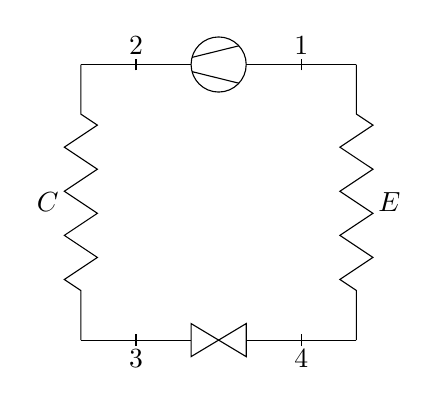
\begin{tikzpicture}[scale=0.7]
		\draw (0,0) -- (2,0) node[midway]{\rule{.4pt}{1ex}} node[midway,below]{3};
		\draw (2,-0.3) -- (2,0.3) -- (3,-0.3) -- (3,0.3) -- cycle;
		\draw (3,0) -- (5,0) node[midway]{\rule{.4pt}{1ex}} node[midway,below]{4};
		\draw (5.6,2.5) node{$E$};
		\draw (5,0) -- (5,0.9) -- (4.7,1.1) -- (5.3,1.5) -- (4.7,1.9) -- (5.3,2.3) -- (4.7,2.7) -- (5.3,3.1) -- (4.7,3.5) -- (5.3,3.9) -- (5,4.1) -- (5,5);
		\draw (2.02,5.13) -- (2.87,5.34);
		\draw (2.02,4.87) -- (2.87,4.66);
		\draw (5,5) -- (3,5) node[midway]{\rule{.4pt}{1ex}} node[midway,above]{1};
		\draw (2.5,5) circle (0.5);
		\draw (2,5) -- (0,5) node[midway]{\rule{.4pt}{1ex}} node[midway,above]{2};
		\draw (-0.6,2.5) node{$C$};
		\draw (0,0) -- (0,0.9) -- (-0.3,1.1) -- (0.3,1.5) -- (-0.3,1.9) -- (0.3,2.3) -- (-0.3,2.7) -- (0.3,3.1) -- (-0.3,3.5) -- (0.3,3.9) -- (0,4.1) -- (0,5);
	\end{tikzpicture}
	\caption{Schéma d'un cycle frigorifique simple}
	\label{fig:simplefrig}
\end{figure}

\begin{figure}[p]\centering
	\tikzsetnextfilename{diagramme_lnp_h}
    \begin{tikzpicture}
        \begin{axis}[
        	enlargelimits=true,
        	grid=major,
        	ymode=log,
        	axis lines=left, xtick=\empty, ytick=\empty,
        	xmin=0,xmax=3500,
        	ylabel=$\ln p$,
        	xlabel=$h$,
		]
			\addplot[black] table[col sep=comma,x index = {1}, y index = {0}] {data/lnp-h.csv};
			\addplot[black] table[col sep=comma,x index = {2}, y index = {0}] {data/lnp-h.csv};
			\draw[thick,red] (3300,1) node{$\bullet$} node[above right]{2} -- (762.5,1) node{$\bullet$} node[above left]{3} -- (762.5,0.01) node{$\bullet$} node[below left]{4} -- (2583.9,0.01) node{$\bullet$} node[below right]{1} to[bend left=-10] cycle;
        \end{axis}
    \end{tikzpicture}
    \caption{Diagramme ($h$,$\ln p$) d'un cycle frigorifique simple}
    \label{fig:diag_h_lnp}
\end{figure}

\subsection{Pourquoi faut-il choisir un fluide frigorigène dont la chaleur massique de la vapeur soit la plus faible possible ?}
Il en va de l'efficacité du cycle frigorifique. Le COP sera d'autant plus élevé que pour $Q_I$ fixé, on aura $W$ faible. Or :
\begin{equation} W = h_2-h_1 = c_PT_1\left[\left(\frac{p_2}{p_1}\right)^{\frac{k-1}{k}}-1\right] \end{equation}
et le rapport de compression $p_2/p_1$ est à peu près indépendant du fluide frigorigène choisi. En conséquence, il faudra choisir un fluide dont le $c_p$ soit la plus faible possible. 

\subsection{Donnez 5 critères technologiques, opérationnels et économiques de choix d'un fluide frigorigène.}
\begin{description}
\item[Coût du compresseur] : le coût est directement lié au débit volumique de fluide frigorigène en $1$. Soit $\dot{P}$ le débit massique de fluide frigorigène, on trouve :
\begin{equation} COP = \frac{\dot{P}Q_I}{\dot{P}W} = \frac{\dot{P}Q_I}{\rho_1\dot{V}_1W} \end{equation} 
Un bon indice de coût est le débit volumique de fluide frigorigène rapporté à l'unité de puissance frigorifique utile, soit :
\begin{equation} \text{coût compresseur } \simeq \frac{\dot{V}_1}{\dot{P}Q_I} = \frac{1}{\rho_1(h_1-h_4)} \end{equation}
On cherche donc un fluide frigorigène avec un grand $\rho$ et donc avec un poids moléculaire élevé.
\item[Pression $p_2$] : le coût de construction de la machine sera évidemment d'autant plus réduit que $p_2$ est modéré.
\item[Pression $p_4=p_1$] : il est important que la pression inférieure du cycle demeure légèrement supérieure à la pression atmosphérique. Il est préférable d'avoir une fuite qu'une rentrée d'air qui obligerait une purge complète et difficile de l'installation.
\item[Viscosité] : elle doit être faible, pour réduire les pertes par frottement et améliorer le transfert de chaleur.
\item[Conductivité thermique] : elle doit être élevée pour réduire la résistance thermique dans la couche limite en contact avec la paroi.
\item[Vitesse du son] : elle doit être élevée afin de permettre des vitesses du fluide très élevée dans le compresseur rotatif (uniquement pour des installations de grandes dimensions.
\item[Compatibilité] : avec l'huile de lubrification du compressuer et avec les matériaux du circuit. Exemple : l'ammoniac est incompatible avec le cuivre.
\item[Stabilité chimique] : la stabilité chimique permet des températures élevées en sortie du compresseur et réduit la déterioration du fluide dans le temps.
\item[Prix du fluide] : pas besoin d'explications.
\end{description}

\subsection{Pourquoi et comment est-ce qu'on réalise le sous-refroidissement du fluide frigorigène au condenseur ?\label{ssec:sous-refroidissement}}
Il est impératif, pour le bon fonctionnement de la machine frigorifique que la condensation du fluide frigorigène soit complète. Soit le cycle frigorifique (1-2-3-4-1) avec condensation complète à la figure \ref{fig:sousrefroid}. Supposons que la condensation soit franchement incomplète pour se terminer en A par exemple, (1-2-A-B-1). Le COP sera considérablement réduit car, si le travail de compression $(h_2-h_1)$ reste identique, l'effet utile $(h_1-h_B)$ lui, aura diminué :
\begin{equation} COP_{12AB} < COP_{1234} \end{equation}
Pour veiller au bon achèvement de la condensation, on se résout à prolonger la condensation par un sous-refroidissement du liquide saturé jusqu'au point 5, dont la température est légèrement inférieure à la température de condensation. Dans ce cas, le sous-refroidissement peut être obtenu grâce au fluide extérieur de refroidissement, par un surdimensionnement de la surface d'échange au condenseur. Un sous-refroidissement plus important peut être obtenu par échange interne à l'aide d'un échangeur additionnel (voir question suivante). 

Il est important de noter qu'un refroidissement effectué de la première manière (surdimensionnement) n'est pas favorable du point de vue des performances thermodynamiques. Le cycle (1-2-5-6-1) a effectivement un meilleur COP que le cycle (1-2-3-4-1), mais les températures de saturation au condenseur ne sont pas les mêmes. Si on compare le COP du cycle (1-2-5-6-1) avec celui du cycle (1-2'-5'-6-1) qui atteint la même température de saturation au condenseur, on observe :
\begin{equation} COP_{1256} < COP_{12'5'6} \end{equation}  
La pratique d'un sous-refroidissement, bien que nécessaire, est donc toujours défavorable du point de vue des performances thermodynamiques.

\begin{figure}[p]\centering
	\tikzsetnextfilename{sousRefroidissement}
    \begin{tikzpicture}
        \begin{axis}[
        	enlargelimits=true,
        	grid=major,
        	ymode=log,
        	axis lines=left, xtick=\empty, ytick=\empty,
        	xmin=0,xmax=3500,
        	ylabel=$\ln p$,
        	xlabel=$h$,
		]
			\addplot[black] table[col sep=comma,x index = {1}, y index = {0}] {data/lnp-h.csv};
			\addplot[black] table[col sep=comma,x index = {2}, y index = {0}] {data/lnp-h.csv};
			\draw[thick,red] (3300,1) node{$\bullet$} node[above right]{2} -- (762.5,1) node{$\bullet$} node[above]{3} -- (762.5,0.01) node{$\bullet$} node[below]{4} -- (2583.9,0.01) node{$\bullet$} node[below right]{1} to[bend left=-10] cycle;
			\draw[red] (1500,1) node{$\circ$} node[above]{$A$} -- (1500,0.01) node{$\circ$} node[below]{$B$};
			\draw[red] (762.5,1) -- (561.4,1) node{$\circ$} node[above]{$5$} -- (561.4,0.01) node{$\circ$} node[below]{$6$} -- (762.5,0.01);
			\draw[red] (762.5,1) -- (300,1) node{$\circ$} node[above]{$7$} -- (300,0.01) node{$\circ$} node[below]{$8$} -- (762.5,0.01);
			\draw[red] (561.4,0.3) node{$\circ$} node[left]{$5'$} -- (3180,0.3) node{$\circ$} node[right]{$2'$};
        \end{axis}
    \end{tikzpicture}
    \caption{Diagrammes ($h$,$\ln p$) de cycles frigorifiques simples (1-2-3-4-1) et (1-2'-5'-6-1), de cycles frigorifiques avec sous-refroidissement (1-2-5-6-1) et (1-2-7-8-1) et d'un cycle à condensation incomplète (1-2-A-B-1)}
    \label{fig:sousrefroid}
\end{figure}

\subsection{Expliquez pourquoi le coefficient de performance (COP) d'une installation frigorifique est indépendant d'un sous-refroidissement à l'aide d'un échangeur de chaleur additionnel.}
Le schéma d'une telle installation est disponible à la figure \ref{fig:frigoechangeur} et le diagramme $(h,\ln p)$ à la figure \ref{fig:sousrefroid}. La chaleur $\Delta Q$ échangée dans l'échangeur $E$ vaut :
\begin{equation} \Delta Q = h_3 - h_7 = h_4-h_8 \end{equation}
En fonctionnement normal (état 3 saturé), le coefficient de performance 
\begin{equation} COP = \frac{h_1-h_4}{h_2-h_1} \end{equation}
demeure indépendant de l'ampleur du sous-refroidissement grâce à l'égalité des longueurs des segments 73 et 84 et est égal à celui du cycle de référence (1-2-3-4-1).

\begin{figure}[p]\centering
	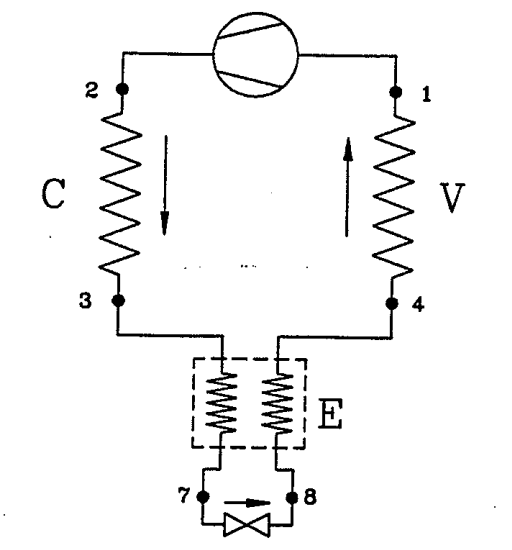
\includegraphics[height=7cm]{figures/frigoechangeur}
	\caption{Installation frigorifique à sous-refroidissement par échangeur de chaleur additionnel}
	\label{fig:frigoechangeur}
\end{figure}

\subsection{Quel est l'état désirable du fluide frigorigène à l'entrée du compresseur d'une installation frigorifique ? Comment peut-on contrôler cet état ?}
La présence de gouttelettes de liquide à l'aspiration du compresseur dégrade significativement son rendement. Un titre inférieur à 1 à l'entrée du compresseur est donc à éviter. À l'opposé, une surchauffe initiale accroît le travail moteur et dégrade donc le COP. 

Le choix le plus favorable est donc l'état saturé.

Pour les grosses installations, la configuration de la figure \ref{fig:grosfrigo} permet d'atteindre simplement le contrôle de cet état, par l'adjonction d'un séparateur $S$ à la sortie de l'évaporateur. On a également ajouté un dispositif optionnel $A$ qui, par effet d'éjection à la sortie du détendeur, permet d'intensifier la circulation naturelle dans l'évaporateur.

Pour les petites installations on adopte la disposition représentée à la figure \ref{fig:petitfrigo} : deux comparateurs de températures $CT1$ et $CT2$ permettent de vérifier en permanence, par l'existence de petits écarts de température, que l'évaporation et la condensation sont bien complètes. 

\begin{figure}[p]\centering
	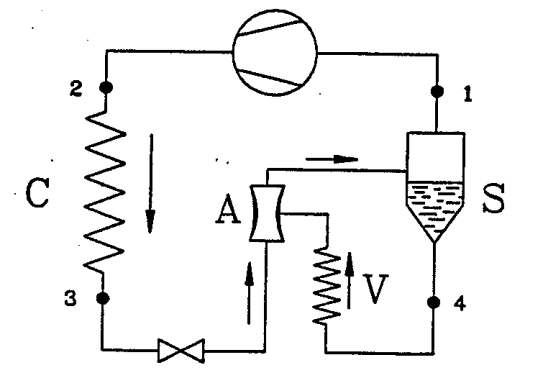
\includegraphics[height=5cm]{figures/grosfrigo}
	\caption{Installation frigorifique avec séparateur}
	\label{fig:grosfrigo}
\end{figure}
\begin{figure}[p]\centering
	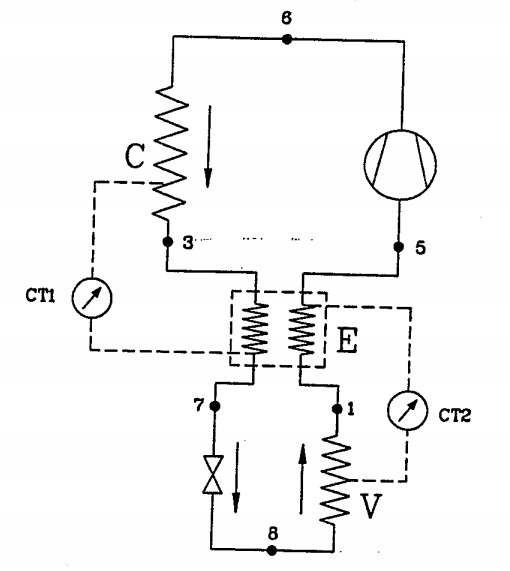
\includegraphics[height=7cm]{figures/petitfrigo}
	\caption{Installation frigorifique avec comparateurs de températures}
	\label{fig:petitfrigo}
\end{figure}

\subsection{Dérivez l'expression du coefficient de performance (COP) pour une pompe à chaleur.}
Une pompe à chaleur est constituée des mêmes organes qu'une machine frigorifique, mais son but est différent : son effet utile sera la production de chaleur au condenseur $C$ par prélèvement de chaleur à l'ambiance au moyen de l'évaporateur $V$ (voir figure \ref{fig:simplefrig} et \ref{fig:diag_h_lnp}).
L'effet utile est donc :
\begin{equation} |Q_{II}| h_2-h_3 \end{equation}
Le travail de compression reste le même que pour une installation frigorifique :
\begin{equation} W = h_2-h_1 \end{equation}
On a donc le coefficient de performance 
\begin{equation} COP = \frac{|Q_{II}|}{W} = \frac{h_2-h_3}{h_2-h_1} \end{equation}
Comme on a, par bilan d'énergie :
\begin{equation} Q_I + W = |Q_{II}| \end{equation}
On peut encore écrire :
\begin{equation} COP = 1 + \frac{Q_I}{W} \end{equation}
